\documentclass{beamer}
\usepackage[utf8]{inputenc}
\usepackage{graphicx, epsfig}
\usepackage{amsmath,mathrsfs,amsfonts,amssymb}
%\usepackage{subfig}
\usepackage{floatflt}
\usepackage{epic,ecltree}
\usepackage{mathtext}
\usepackage{fancybox}
\usepackage{fancyhdr}
\usepackage{multirow}
\usepackage{enumerate}
\usepackage{epstopdf}
\usepackage{multicol}
\usepackage{algorithm}
\usepackage[noend]{algorithmic}
\usepackage{tikz}
\usepackage{blindtext}
\usetheme{default}%{Singapore}%{Warsaw}%{Warsaw}%{Darmstadt}
\usecolortheme{default}
\setbeamerfont{title}{size=\Huge}
\setbeamertemplate{footline}[page number]{}


\makeatletter
\newcommand\HUGE{\@setfontsize\Huge{35}{40}}
\makeatother    

\setbeamerfont{title}{size=\HUGE}
\beamertemplatenavigationsymbolsempty

% latin bold lower
\newcommand{\ba}{\mathbf{a}} 
\newcommand{\bc}{\mathbf{c}} 
\newcommand{\be}{\mathbf{e}} 
\newcommand{\bh}{\mathbf{h}} 
\newcommand{\bp}{\mathbf{p}} 
\newcommand{\bt}{\mathbf{t}} 
\newcommand{\bs}{\mathbf{s}} 
\newcommand{\bu}{\mathbf{u}} 
\newcommand{\bv}{\mathbf{v}} 
\newcommand{\bw}{\mathbf{w}} 
\newcommand{\bx}{\mathbf{x}} 
\newcommand{\by}{\mathbf{y}} 
\newcommand{\bz}{\mathbf{z}} 

% latin bold upper
\newcommand{\bA}{\mathbf{A}} 
\newcommand{\bB}{\mathbf{B}} 
\newcommand{\bC}{\mathbf{C}} 
\newcommand{\bI}{\mathbf{I}} 
\newcommand{\bL}{\mathbf{L}} 
\newcommand{\bM}{\mathbf{M}} 
\newcommand{\bQ}{\mathbf{Q}} 
\newcommand{\bT}{\mathbf{T}} 
\newcommand{\bU}{\mathbf{U}} 
\newcommand{\bV}{\mathbf{V}} 
\newcommand{\bW}{\mathbf{W}} 
\newcommand{\bX}{\mathbf{X}} 
\newcommand{\bY}{\mathbf{Y}} 
\newcommand{\bZ}{\mathbf{Z}} 

% latin cal upper
\newcommand{\cG}{\mathcal{G}} 
\newcommand{\cL}{\mathcal{L}} 
\newcommand{\cN}{\mathcal{N}} 
\newcommand{\cS}{\mathcal{S}} 
\newcommand{\cT}{\mathcal{T}} 
\newcommand{\cW}{\mathcal{W}} 
\newcommand{\cX}{\mathcal{X}} 
\newcommand{\cZ}{\mathcal{Z}} 

% latin bb upper
\newcommand{\bbE}{\mathbb{E}} 
\newcommand{\bbI}{\mathbb{I}} 
\newcommand{\bbP}{\mathbb{P}} 
\newcommand{\bbR}{\mathbb{R}} 

% greek bold lower
\newcommand{\bepsilon}{\boldsymbol{\epsilon}} 
\newcommand{\btheta}{\boldsymbol{\theta}} 
\newcommand{\blambda}{\boldsymbol{\lambda}} 
\newcommand{\bpi}{\boldsymbol{\pi}} 
\newcommand{\bmu}{\boldsymbol{\mu}} 
\newcommand{\bsigma}{\boldsymbol{\sigma}} 
\newcommand{\bphi}{\boldsymbol{\phi}} 

% greek bold upper
\newcommand{\bSigma}{\boldsymbol{\Sigma}} 

\DeclareMathOperator*{\argmin}{arg\,min}
\DeclareMathOperator*{\argmax}{arg\,max}

\newcommand{\createdgmtitle}[1]{\title[\hbox to 56mm{Deep Generative Models  \hfill\insertframenumber\,/\,\inserttotalframenumber}]
	{\vspace{1.5cm} \\ Deep Generative Models \\ {\Huge Lecture #1}}
	\author{Roman Isachenko}
	\institute{
	Moscow Institute of Physics and Technology
	} 
	\date{Autumn, 2021}
}

\newcommand\myfootnote[1]{%
  \tikz[remember picture,overlay]
  \draw (current page.south west) +(1in + \oddsidemargin,0.5em)
  node[anchor=south west,inner sep=0pt]{\parbox{\textwidth}{%
      \rlap{\rule{10em}{0.4pt}}\raggedright\scriptsize \textit{#1}}};}

\newcommand\myfootnotewithlink[2]{%
  \tikz[remember picture,overlay]
  \draw (current page.south west) +(1in + \oddsidemargin,0.5em)
  node[anchor=south west,inner sep=0pt]{\parbox{\textwidth}{%
      \rlap{\rule{10em}{0.4pt}}\raggedright\scriptsize\href{#1}{\textit{#2}}}};}
\createdgmtitle{4}
%--------------------------------------------------------------------------------
\begin{document}
%--------------------------------------------------------------------------------
\begin{frame}
%\thispagestyle{empty}
\titlepage
\end{frame}
%=======
\begin{frame}{VAE limitations}
	\begin{itemize}
		\item Poor variational posterior distribution (inference model encoder)
		\[
		q(\bz | \bx, \bphi) = \mathcal{N}(\bz| \bmu_{\bphi}(\bx), \bsigma^2_{\bphi}(\bx)).
		\]
		\item Poor prior distribution
		\[
		p(\bz) = \mathcal{N}(0, \mathbf{I}).
		\]
		\item Poor probabilistic model (generative model, decoder)
		\[
		p(\bx | \bz, \btheta) = \mathcal{N}(\bx| \bmu_{\btheta}(\bz), \bsigma^2_{\btheta}(\bz)).
		\]
		\item Loose lower bound
		\[
		\log p(\bx | \btheta) - \mathcal{L}(q, \btheta) = (?).
		\]
	\end{itemize}
\end{frame}
%=======
\begin{frame}{Bayesian framework}
	\begin{block}{Bayes theorem}
		\[
			p(\bt | \bx) = \frac{p(\bx | \bt) p(\bt)}{p(\bx)} = \frac{p(\bx | \bt) p(\bt)}{\int p(\bx | \bt) p(\bt) d \bt} 
		\]
		\begin{itemize}
			\item $\bx$ -- observed variables, $\bt$ -- unobserved variables (latent variables/parameters);
			\item $p(\bx | \bt)$ -- likelihood;
			\item $p(\bx) = \int p(\bx | \bt) p(\bt) d \bt$ -- evidence;
			\item $p(\bt)$ -- prior distribution, $p(\bt | \bx)$ -- posterior distribution.
		\end{itemize}
	\end{block}
	\begin{block}{Meaning}
		We have unobserved variables $\bt$ and some prior knowledge about them $p(\bt)$. Then, the data $\bx$ has been observed. 
		Posterior distribution $p(\bt | \bx)$ summarizes the knowledge after the observations.
	\end{block}
\end{frame}
%=======
\begin{frame}{Variational Lower Bound}
    We have set of objects $\bX = \{\bx_i\}_{i=1}^n$. 
    The goal is to perform Bayesian inference on the unobserved variables $\bT = \{\bt_i\}_{i=1}^n$.
    \begin{block}{Evidence Lower Bound (ELBO)}
    \vspace{-0.3cm}
        \begin{multline*}
    		\log p(\bX) 
    		= \log \frac{p(\bX, \bT)}{p(\bT|\bX)} = \\ 
    		= \int q(\bT) \log \frac{p(\bX, \bT)}{p(\bT|\bX)}d\bT
    		= \int q(\bT) \log \frac{p(\bX, \bT) q(\bT)}{p(\bT|\bX) q(\bT)} d\bT = \\
    		= \int q(\bT) \log \frac{p(\bX, \bT)}{q(\bT)}d\bT + \int q(\bT) \log \frac{q(\bT)}{p(\bT|\bX)}d\bT = \\ 
    		= \mathcal{L} (q) + KL(q(\bT) || p(\bT|\bX)) \geq \mathcal{L} (q).
    	\end{multline*}
        \vspace{-0.3cm}
    \end{block}
	We would like to maximize lower bound $\mathcal{L}(q)$.
\end{frame}
%=======
\begin{frame}{Mean field approximation}
    \begin{block}{Independence assumption}
    \vspace{-0.3cm}
    \[
    q(\bT) = \prod_{i=1}^k q_i(\bT_i), \quad \bT = [\bT_1, \dots, \bT_k], \, \bT_j = \{ \bt_{ij}\}_{i=1}^n, \, \bt_i = \{ \bT_{ij}\}_{j=1}^k.
    \]
    \vspace{-0.3cm}
    \end{block}
    \begin{block}{Block coordinate optimization of ELBO for $q_j(\bT_j)$}
  
    {\footnotesize
    \vspace{-0.3cm}
        \begin{multline*}
    		\mathcal{L} (q)
    		= \int q(\bT) \log \frac{p(\bX, \bT)}{q(\bT)}d\bT
    		= \int \left[\prod_{i=1}^k q_i(\bT_i) \right] \log \frac{p(\bX, \bT)}{\left[\prod_{i=1}^k q_i(\bT_i) \right]}  \prod_{i=1}^k d \bT_i = \\
    		= \int \left[ \prod_{i=1}^k q_i \right] \log p(\bX, \bT) \prod_{i=1}^k d \bT_i  
    		- \sum_{i=1}^k \int \left[ \prod_{j=1}^k q_j \right] \log q_i \prod_{j=1}^k d \bT_j = \\
    		= \int q_j \left[\int  \log p(\bX, \bT) \prod_{i \neq j} q_i d \bT_i \right] d \bT_j - \\
    		- \int q_j \log q_j d\bT_j + \text{const}(q_j) \rightarrow \max_{q_j}
    	\end{multline*}
        \vspace{-0.3cm}}
    \end{block}
\end{frame}
%=======
\begin{frame}{Mean field approximation}
	\footnotesize
	\begin{block}{Block coordinate optimization of ELBO for $q_j(\bT_j)$}
		\vspace{-0.4cm}
	    \begin{multline*}
			\mathcal{L} (q) 
			= \int q_j \left[\int \log p(\bX, \bT) \prod_{i \neq j} q_i d \bT_i \right] d \bT_j
			- \int q_j \log q_j  d\bT_j + \text{const}(q_j) = \\
			= \int q_j \log \hat{p}(\bX, \bT_j) d \bT_j 
			- \int q_j \log q_j d\bT_j + \text{const}(q_j) \rightarrow \max_{q_j}.
		\end{multline*}
		Here we introduce
		\[
		   \log \hat{p}(\bX, \bT_j) = \int \log p(\bX, \bT) \prod_{i \neq j} q_i d \bT_i = \mathbb{E}_{i \neq j} \log p(\bX, \bT) + \text{const}(q_j)
		\]
	    \end{block}
	    \vspace{-0.3cm}
	    \begin{block}{Final ELBO derivation for $q_j(\bT_j)$}
	    	\vspace{-0.5cm}
			\begin{multline*}
	    		\mathcal{L} (q)
	    		= \int q_j (\bT_j) \log \hat{p}(\bX, \bT_j) d \bT_j - \int q_j(\bT_j) \log q_j(\bT_j) d\bT_j + \text{const}(q_j) = \\
	    		 \int q_j (\bT_j) \log \frac{\hat{p}(\bX, \bT_j)}{q_j(\bT_j)} d\bT_j + \text{const}(q_j) = \\
	    		= - KL (q_j(\bT_j) || \hat{p}(\bX, \bT_j)) + \text{const}(q_j) \rightarrow \max_{q_j}.
	    	\end{multline*}
	    \end{block}
\end{frame}
%=======    
\begin{frame}{Mean field approximation}   
	 \begin{block}{Independence assumption}
		\vspace{-0.3cm}
		\[
		q(\bT) = \prod_{i=1}^k q_i(\bT_i), \quad \bT = [\bT_1, \dots, \bT_k], \quad \bT_j = \{ \bt_{ij}\}_{i=1}^n.
		\]
		\vspace{-0.3cm}
	\end{block}
	\begin{block}{ELBO}
	    \[
			\mathcal{L} (q) = - KL (q_j(\bT_j) || \hat{p}(\bX, \bT_j))  + \text{const}(q_j) \rightarrow \max_{q_j}.
	    \]
	    \vspace{-0.3cm}
	\end{block}
	 \begin{block}{Solution}
	 	\vspace{-0.3cm}
		 \[
		    q_j(\bT_j) = \text{const} \cdot \hat{p}(\bX, \bT_j)
		 \]
		 \[
		 	\log \hat{p}(\bX, \bT_j) = \mathbb{E}_{i \neq j} \log p(\bX, \bT) + \text{const}
		 \]
		 \[
		     \log q_j(\bT_j) = \mathbb{E}_{i \neq j} \log p(\bX, \bT) + \text{const}
		 \]
		 \vspace{-0.3cm}
	 \end{block}
\end{frame}
%=======
\begin{frame}{Mean field approximation}
	\begin{block}{ELBO}
		\[
			\mathcal{L} (q) = - KL (q_j(\bT_j) || \hat{p}(\bX, \bT_j))  + \text{const}(q_j) \rightarrow \max_{q_j}.
		\]
		\vspace{-0.3cm}
	\end{block}
	\begin{block}{Solution}
		\vspace{-0.3cm}
		\[
			\log q_j(\bT_j) = \mathbb{E}_{i \neq j} \log p(\bX, \bT) + \text{const}
		\]
		\vspace{-0.3cm}
	\end{block}
	Assumptions: 
	\begin{itemize}
		\item $\bT = [\bT_1, \bT_2] = [\bZ, \btheta]$, $q(\bT) = q(\bT_1) \cdot q(\bT_2) = q(\bZ) \cdot q(\btheta)$.
		\item restrict a class of probability distributions for $\btheta$ to Dirac delta functions:
		\[
			q_2 = q(\bT_2) = q(\btheta) = \delta(\btheta - \btheta^*).
		\]
		
		Under the restrictions the exact solution for $q_2$ is not reached (KL can be greater than 0).
	\end{itemize}
\end{frame}
%=======
\begin{frame}{Mean field approximation}
	\begin{block}{General solution}
		\vspace{-0.3cm}
		\[
		\log q_j(\bT_j) = \mathbb{E}_{i \neq j} \log p(\bX, \bT) + \text{const}
		\]
		\vspace{-0.3cm}
	\end{block}
	\begin{block}{Solution for $q_1 = q(\bZ)$}
		\vspace{-0.3cm}
		\begin{multline*}
			\log q(\bZ) = \int q(\btheta) \log p(\bX, \bZ,  \btheta) d\btheta + \text{const} = \\
			= \int \delta(\btheta - \btheta^*) \log p(\bX, \bZ,  \btheta) d\btheta + \text{const} = \\
			= \log p (\bZ | \bX, \btheta^*) +  \text{const}.
		\end{multline*}
	\end{block}
	\vspace{-0.3cm}
	\begin{block}{EM-algorithm (E-step)}
		\vspace{-0.3cm}
	\[
		q(\bZ) = \argmax_q \mathcal{L} (q, \btheta^*) = \argmin_q KL(q || p) = p(\bZ| \bX, \btheta^*).
	\]
	\end{block}
\end{frame}
%=======
\begin{frame}{Mean field approximation}
	\begin{block}{ELBO}
		\[
			\mathcal{L} (q) = - KL (q_j(\bT_j) || \hat{p}(\bX, \bT_j))  + \text{const}(q_j) \rightarrow \max_{q_j}.
		\]
	\vspace{-0.3cm}
	\end{block}
	\begin{block}{ELBO maximization w.r.t. $q_2 = q(\btheta) = \delta(\btheta - \btheta^*)$}
		\vspace{-0.3cm}
		\begin{align*}
			\mathcal{L} (q_1, q_2) &= - KL (q(\btheta) || \hat{p}(\bX, \btheta))  + \text{const}(\btheta^*) \\ 
			&= \int q (\btheta) \log \frac{\hat{p}(\bX, \btheta)}{q(\btheta)} d\btheta + \text{const}(\btheta^*) \\
			& = \int q (\btheta) \log \hat{p}(\bX, \btheta) d\btheta  - \int q (\btheta) \log q(\btheta) d\btheta + \text{const}(\btheta^*) \\
			& = \int \delta(\btheta - \btheta^*) \log \hat{p}(\bX, \btheta) d\btheta + \text{const}(\btheta^*) \rightarrow \max_{\btheta^*}
		\end{align*}
		\vspace{-0.3cm}
	\end{block}
\end{frame}
%=======
\begin{frame}{Mean field approximation}
	
	\begin{block}{ELBO maximization w.r.t. $q_2 = q(\btheta) = \delta(\btheta - \btheta^*)$}
		\vspace{-0.3cm}
		\begin{multline*}
			\mathcal{L} (q_1, q_2) = \int \delta(\btheta - \btheta^*) \log \hat{p}(\bX, \btheta) d\btheta + \text{const}
			= \log \hat{p}(\bX, \btheta^*)  + \text{const} \\
			= \mathbb{E}_{i \neq j} \log p(\bX, \bT) + \text{const} = \mathbb{E}_{q_1} \log p(\bX, \bZ, \btheta^*) + \text{const} \\
		= \int q(\bZ) \log p(\bX, \bZ|  \btheta^*) d\bZ + \log p(\btheta^*)+ \text{const}\rightarrow \max_{\btheta^*}
	\end{multline*}
	\end{block}
	\vspace{-0.3cm}
	\begin{block}{EM-algorithm (M-step)}
		\vspace{-0.3cm}
		 \begin{align*}
		 	\mathcal{L}(q, \btheta) &= \int q(\bZ) \log \frac{p(\bX, \bZ | \btheta)}{q(\bZ)}d\bZ \\
		 	&= \int q(\bZ) \log p(\bX, \bZ | \btheta) d\bZ + \text{const} \rightarrow \max_{\btheta}
		 \end{align*}
	\end{block}
\end{frame}
%=======
\begin{frame}{Mean field approximation}
    \begin{block}{Solution}
    \[
        \log q_j(\bT_j) = \mathbb{E}_{i \neq j} \log p(\bX, \bT) + \text{const}
    \]
    \end{block}

	\begin{block}{EM algorithm (special case)}
	\begin{itemize}
		\item Initialize $\btheta^*$;
		\item E-step
		\[
			q(\bZ) = \argmax_q \mathcal{L} (q, \btheta^*) = \argmin_q KL(q || p) =
			 p(\bZ| \bX, \btheta^*);
		\]
		\item M-step
		\[
			\btheta^* = \argmax_{\btheta} \mathcal{L} (q, \btheta);
		\]
		\item Repeat E-step and M-step until convergence.
	\end{itemize}
	\end{block}
\end{frame}
%=======
\begin{frame}{Likelihood-based models so far...}
	\begin{minipage}[t]{0.5\columnwidth}
		\begin{block}{Autoregressive models}
			\vspace{-0.5cm}
			\[
			p(\bx|\btheta) = \prod_{i=1}^m p(x_i | \bx_{1:i - 1}, \btheta)
			\]
			\vspace{-0.2cm}
			\begin{itemize}
				\item tractable likelihood, 
				\item no inferred latent factors.
			\end{itemize}
		\end{block}
	\end{minipage}%
	\begin{minipage}[t]{0.5\columnwidth}
		\begin{block}{Latent variable models}
			\[
			p(\bx| \btheta) = \int p(\bx, \bz | \btheta) d \bz
			\]
			\begin{itemize}
				\item latent feature representation, 
				\item intractable likelihood.
			\end{itemize}
		\end{block}
	\end{minipage}
	
	\vspace{1cm } 
	How to build model with latent variables and tractable likelihood?
\end{frame}
%=======
\begin{frame}{Flows intuition}
	Let $\xi$ be a random variable with density $p(\xi)$. Then
	\[
	\eta = F(\xi) = \int_{-\infty}^\xi p(t)dt \sim U[0, 1].
	\]
	\[
		P(\eta < y) = P(F(\xi) < y) = P(\xi < F^{-1}(y)) = F(F^{-1}(y)) = y
	\]
	Hence
	\[
	\eta \sim U[0, 1]; \quad \xi = F^{-1}(\eta) \quad \Rightarrow \quad \xi \sim p(\xi).
	\]
	\begin{figure}
		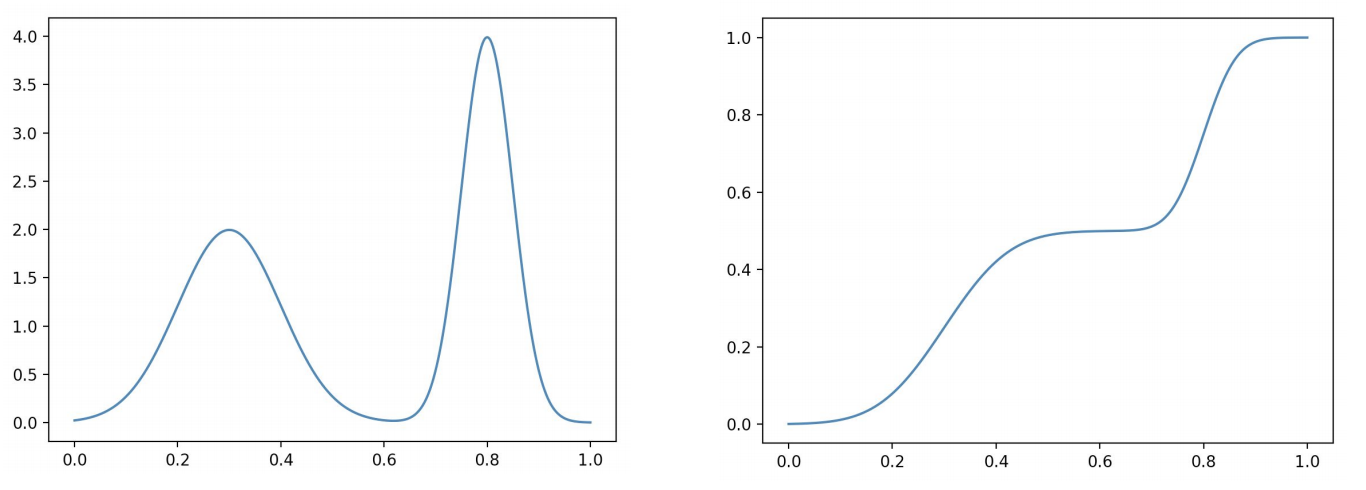
\includegraphics[width=\linewidth]{figs/flows_1d}
	\end{figure}
	\myfootnotewithlink{https://sites.google.com/view/berkeley-cs294-158-sp19/home}{image credit: https://sites.google.com/view/berkeley-cs294-158-sp19/home}
	
\end{frame}
%=======
\begin{frame}{Flows intuition}
	\begin{itemize}
		\item Let $z \sim p(z)$ is a random variable with base distribution $p(z) = U[0, 1]$. 
		\item Let $x \sim p(x)$ is a random variable with complex distribution $p(x)$ and cdf $F(x)$. 
		\item Then noise variable $z$ can be transformed to $x$ using inverse cdf~$F^{-1}$ ($x = F^{-1}(z)$).
	\end{itemize}
	How to transform random variable $z$  which has a distribution different from uniform to $x$?
		\begin{itemize}
			\item Let $z \sim p(z)$ is a random variable with base distribution $p(z)$ and cdf $G(z)$.
			\item Then $z_0 = G(z)$ has base distribution $p(z_0) = U[0, 1]$.
			\item Let $x \sim p(x)$ is a random variable with complex distribution $p(x)$ and cdf $F(x)$. 
			\item Then noise variable $z$ can be transformed to $x$ using cdf $G$ and inverse cdf~$F^{-1}$ ($x = F^{-1}(z_0) = F^{-1}(G(z))$).
		\end{itemize}
\end{frame}
%=======
\begin{frame}{Change of variables}
	\begin{block}{Theorem}
		\begin{itemize}
			\item $\bx$ is a random variable with density function $p(\bx)$;
			\item $f: \mathbb{R}^m \rightarrow \mathbb{R}^m$ is a differentiable, invertible function (diffeomorphism);
			\item $\bz = f(\bx)$, $\bx = f^{-1}(\bz) = g(\bz)$ (here $g = f^{-1}$).
		\end{itemize}
		Then
		\vspace{-0.3cm}
		\begin{align*}
			p(\bx) &= p(\bz) \left|\det \left(  \frac{\partial \bz}{\partial \bx} \right) \right| = p(f(\bx)) \left|\det \left(  \frac{\partial f(\bx)}{\partial \bx} \right) \right| \\
			p(\bz) &= p(\bx) \left|\det \left(  \frac{\partial \bx}{\partial \bz} \right) \right| = p(g(\bz)) \left|\det \left(  \frac{\partial g(\bz)}{\partial \bz} \right) \right|.
		\end{align*}
	\end{block}
		\begin{itemize}
			\item $\bx$ and $\bz$ have the same dimensionality (lies in $\bbR^m$);
			\item $ \left|\det \left(  \frac{\partial f(\bx)}{\partial \bx} \right)\right| = \left|\det \left(  \frac{\partial g^{-1}(\bx)}{\partial \bx} \right)\right| = \left|\det \left(  \frac{\partial g(\bz)}{\partial \bz} \right)\right|^{-1}$;
			\item $f(\bx, \btheta)$ could be parametric function.
		\end{itemize}
\end{frame}
%=======
\begin{frame}{Fitting flows}
	\begin{block}{MLE problem}
		\vspace{-0.3cm}
		\[
		\btheta^* = \argmax_{\btheta} p(\bX | \btheta) = \argmax_{\btheta} \prod_{i=1}^n p(\bx_i | \btheta) = \argmax_{\btheta} \sum_{i=1}^n \log p(\bx_i | \btheta).
		\]
		\vspace{-0.3cm}
	\end{block}
	\begin{block}{Challenge}
		$p(\bx | \btheta)$ can be intractable.
	\end{block}
	\begin{block}{Fitting flow to solve MLE}
		\[
		p(\bx|\btheta) = p(\bz) \left|\det \left(  \frac{\partial \bz}{\partial \bx} \right) \right|  = p(f(\bx, \btheta)) \left|\det \left( \frac{\partial f(\bx, \btheta)}{\partial \bx} \right) \right|
		\]
		\[
			\log p(\bx|\btheta) = \log p(f(\bx, \btheta)) + \log  \left|\det \left( \frac{\partial f(\bx, \btheta)}{\partial \bx} \right) \right|
		\]
	\end{block}
\end{frame}
%=======
\begin{frame}{Flows}
	\begin{figure}
		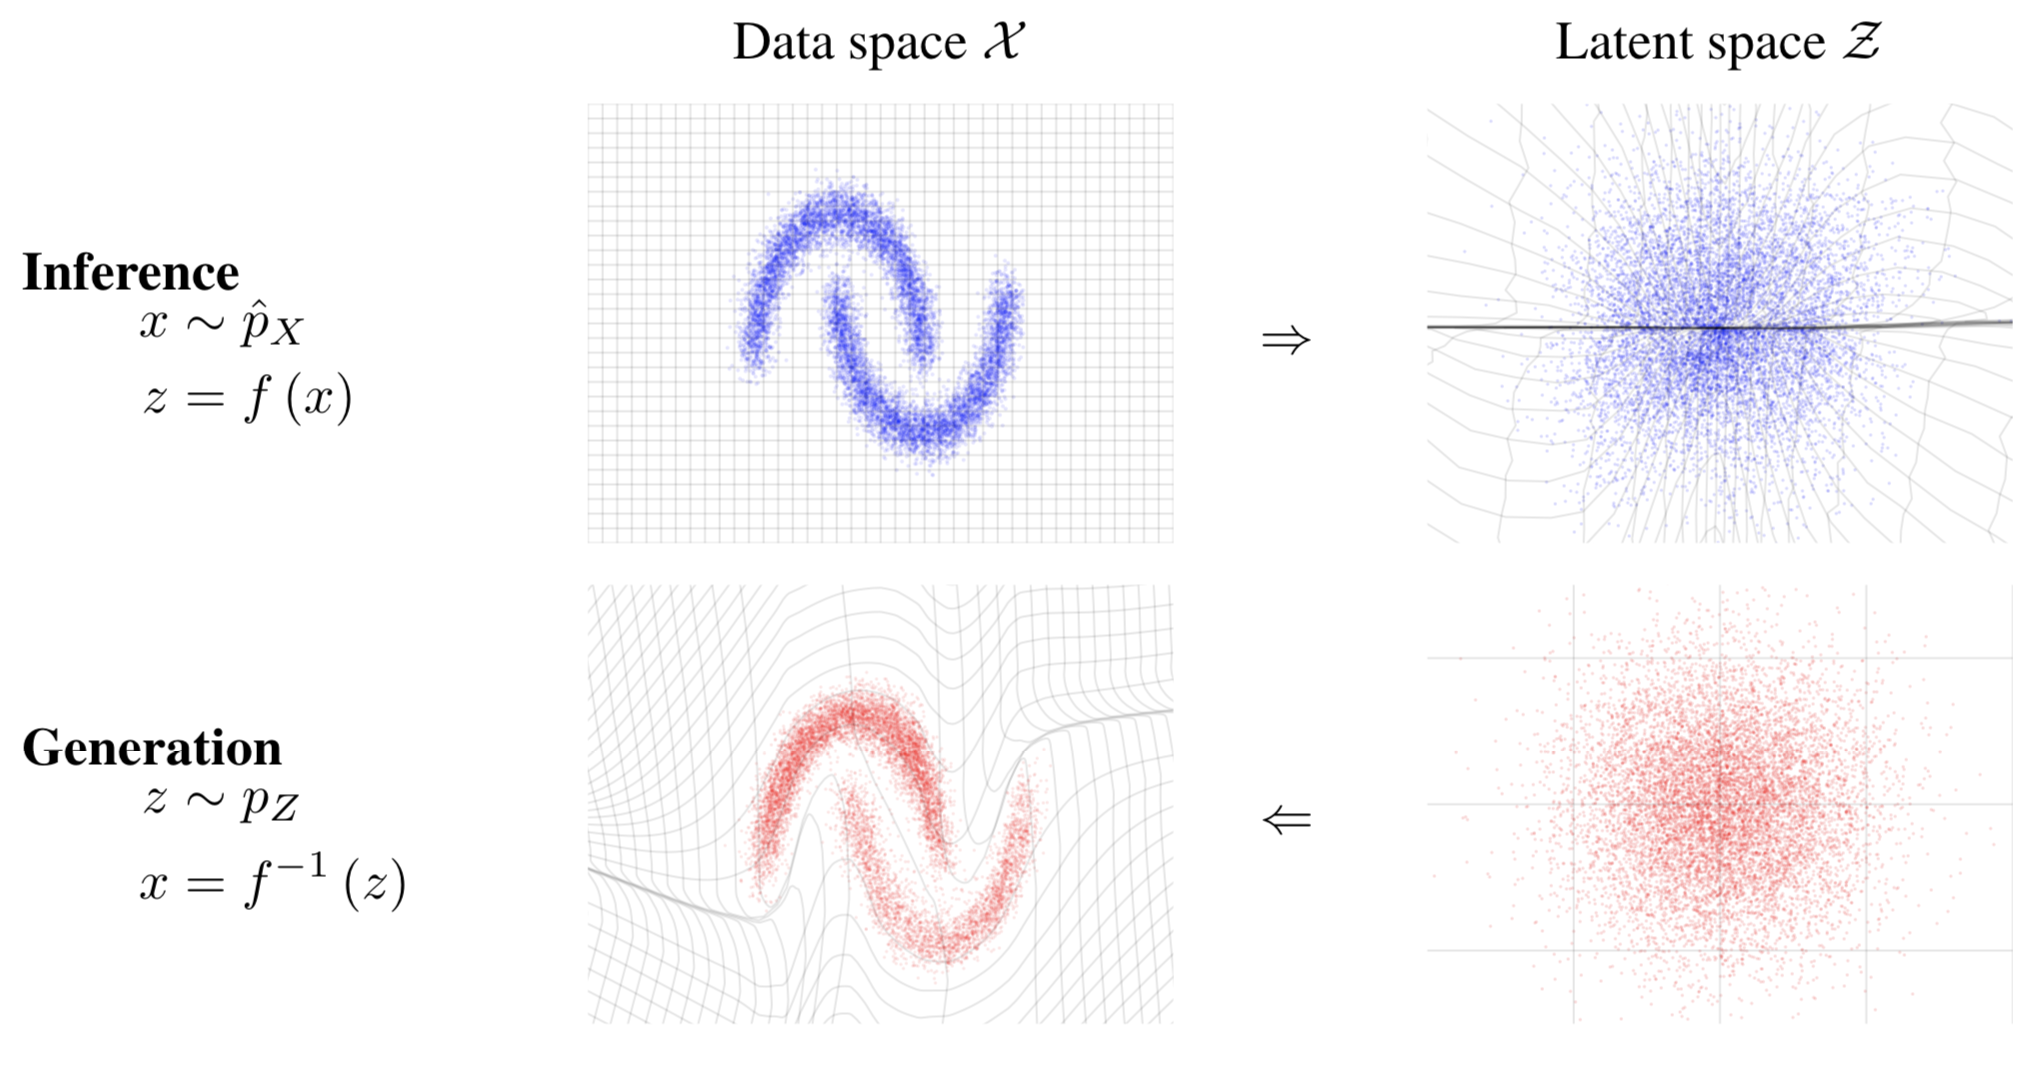
\includegraphics[width=0.7\linewidth]{figs/flows_how2.png}
	\end{figure}
	\vspace{-0.3cm}
	\begin{block}{Computational requirement}
		\begin{itemize}	
			\item Evaluating model density $p(\bx | \btheta)$ requires computing the transformation $\bz = f(\bx,  \btheta)$ and its Jacobian determinant $\left|\det \left( \frac{\partial f(\bx, \btheta)}{\partial \bx} \right) \right|$,
			and evaluating the density $p(\bz)$.
			\item Sampling $\bx$ from the model requires the ability to sample from $p(\bz)$ and to compute the transformation $\bx = g(\bz, \btheta) = f^{-1}(\bz, \btheta)$. 
		\end{itemize}
	\end{block}
	\myfootnotewithlink{https://arxiv.org/abs/1605.08803}{Dinh L., Sohl-Dickstein J., Bengio S. Density estimation using Real NVP, 2016} 
\end{frame}
%=======
\begin{frame}{Forward KL vs Reverse KL}
	Fix probabilistic model $p(\bx | \btheta)$~-- the set of parameterized distributions . \\
	Instead of searching true $\pi(\bx)$ over all probability distributions, learn function approximation $p(\bx | \btheta) \approx \pi(\bx)$.
	\begin{block}{Forward KL}
		\vspace{-0.2cm}
		\[
			KL(\pi || p) = \int \pi (\bx) \log \frac{\pi(\bx)}{p(\bx | \btheta)} d \bx \rightarrow \min_{\btheta}
		\]
	\end{block}
	\begin{block}{Reverse KL}
		\vspace{-0.2cm}
		\[
			KL(p || \pi) = \int p (\bx| \btheta) \log \frac{p(\bx| \btheta)}{\pi(\bx)} d \bx \rightarrow \min_{\btheta}
		\]
	\end{block}
	\begin{itemize}
		\item What is the difference between these two formulations?
		\item What do we get in these two cases if $p(\bx | \btheta)$ is a flow model?
	\end{itemize}
\end{frame}
%=======
\begin{frame}{Forward KL vs Reverse KL}
	\begin{block}{Forward KL}
		    \vspace{-0.5cm}
		\begin{align*}
			KL(\pi || p) &= \int \pi (\bx) \log \frac{\pi(\bx)}{p(\bx | \btheta)} d \bx \\
			&= \int \pi (\bx) \log \pi(\bx) d \bx - \int \pi (\bx) \log p(\bx | \btheta) d \bx \\
			&= - \bbE_{\pi(\bx)} \log p(\bx | \btheta) + \text{const} \rightarrow \min_{\btheta}
		\end{align*}
		\vspace{-0.5cm}
	\end{block}
	\begin{block}{Monte-Carlo estimation}
		\vspace{-0.5cm}
		\[
			KL(\pi || p) = - \bbE_{\pi(\bx)} \log p(\bx | \btheta) + \text{const} \approx - \frac{1}{n} \sum_{i=1}^n \log p(\bx_i | \btheta) \rightarrow \min_{\btheta}.
		\]
		\vspace{-0.5cm}
	\end{block}
	    \begin{block}{MLE problem}
	    \vspace{-0.5cm}
	    \[
	        \btheta^* = \argmax_{\btheta} p(\bX | \btheta) = \argmax_{\btheta} \prod_{i=1}^n p(\bx_i | \btheta) = \argmax_{\btheta} \sum_{i=1}^n \log p(\bx_i | \btheta).
	    \]
	    \vspace{-0.1cm}
	    \end{block}
\end{frame}
%=======
\begin{frame}{Forward KL vs Reverse KL}
	\begin{block}{Forward KL}
	    \vspace{-0.3cm}
		\[
			\btheta^* = \argmax_{\btheta} \frac{1}{n} \sum_{i=1}^n \log p(\bx_i | \btheta) \approx  \argmin_{\btheta} KL(\pi || p)
		\]
		Maximum likelihood estimation is equivalent to minimization of the Monte-Carlo estimation of forward KL.
	\end{block}
	\begin{block}{Forward KL for flow model}
	    \vspace{-0.3cm}
		\[
			\log p(\bx|\btheta) = \log p(f(\bx, \btheta)) + \log  \left|\det \left( \frac{\partial f(\bx, \btheta)}{\partial \bx} \right) \right|
		\]
		\begin{itemize}
		\item We need to be able to compute $f(\bx, \btheta)$ and its Jacobian.
		\item We need to be able to compute the density $p(\bz)$.
		\item We don’t need to think about computing the function $g(\bz, \btheta) = f^{-1}(\bz, \btheta)$ until we want to sample from the flow.
		\end{itemize}
	\end{block}
\end{frame}
%=======
\begin{frame}{Forward KL vs Reverse KL}
	\begin{block}{Reverse KL}
	  	\vspace{-0.5cm}
			\begin{align*}
				KL(p || \pi) &= \int p(\bx | \btheta) \log \frac{p(\bx | \btheta)}{\pi(\bx)} d \bx \\
				&= \bbE_{p(\bx | \btheta)} \left[\log p(\bx | \btheta) - \log \pi(\bx)\right] \rightarrow \min_{\btheta}
			\end{align*}
		\vspace{-0.7cm}
	\end{block}
	\begin{block}{Reverse KL for flow model}
  		\vspace{-0.3cm}
		\[
			\log p(\bz) = \log p(\bx | \btheta) + \log \left|\det \left( \frac{\partial g(\bz, \btheta)}{\partial \bz} \right) \right|
		\]
		\[
			KL(p || \pi)  = \bbE_{p(\bz)} \left[  \log p(\bz) - \log \left|\det \left( \frac{\partial g(\bz, \btheta)}{\partial \bz} \right) \right| - \log \pi(g(\bz, \btheta)) \right]
		\]
		\begin{itemize}
		\item We need to be able to compute $g(\bz, \btheta)$ and its Jacobian.
		\item We need to be able to sample from the density $p(\bz)$ (do not need to evaluate it).
		\item We don’t need to think about computing the function $f(\bx, \btheta)$.
		\end{itemize}
	\end{block}
\end{frame}
%=======
\begin{frame}{Composition of flows}
	\begin{block}{Theorem}
		Diffeomorphisms are \textbf{composable} (If $f_1, f_2$ satisfy conditions of the change of variable theorem (differentiable and invertible), then $\bz = f(\bx) = f_2 \circ f_1(\bx)$ also satisfies it).
	\end{block}
	\begin{multline*}
		p(\bx) = p(\bz) \left|\det \left(  \frac{\partial \bz}{\partial \bx} \right) \right| = p(f(\bx)) \left|\det \left(  \frac{\partial f(\bx)}{\partial \bx} \right) \right| = \\
		= p(f(\bx)) \left|\det \left(\frac{\partial f_2 \circ f_1(\bx)}{\partial \bx} \right) \right| =
		p(f(\bx)) \left|\det \left(\frac{\partial \textbf{f}_2}{\partial \textbf{f}_1} \cdot \frac{\partial \textbf{f}_1}{\partial \bx} \right) \right| = \\
		= p(f(\bx))  \left|\det \left(\frac{\partial \textbf{f}_2}{\partial \textbf{f}_1} \right) \right| \cdot \left| \det \left( \frac{\partial \textbf{f}_1}{\partial \bx} \right) \right|
	\end{multline*}

	What will we get in the case $\bz = f(\bx) = f_n \circ \dots \circ f_1(\bx)$?
\end{frame}
%=======
\begin{frame}{Flows}
	\vspace{-0.3cm}
	\[
		\log p(\bx|\btheta) = \log p(f(\bx, \btheta)) + \log \left|\det \left( \frac{\partial f(\bx, \btheta)}{\partial \bx} \right) \right|
	\]
	\vspace{-0.3cm}
	\begin{block}{Definition}
		Normalizing flow is a \textit{differentiable, invertible} mapping from data $\bx$ to the noise $\bz$. 
	\end{block}
	\begin{itemize}
		\item "Normalizing" means that the inverse flow takes samples from $p(\bx)$ and normalizes them into samples from density $p(\bz)$.
		\item "Flow" refers to the trajectory followed by samples from $p(\bz)$ as they are transformed by the sequence of transformations
		\[
		\bz = f_K \circ \dots \circ f_1(\bx); \quad \bx = f_1^{-1} \circ \dots \circ f_K^{-1} (\bz) = g_1 \circ \dots \circ g_K(\bz) 
		\] 
		\begin{multline*}
			p(\bx) = p(f_K \circ \dots \circ f_1(\bx)) \left|\det \left(\frac{\partial f_K \circ \dots \circ f_1(\bx)}{\partial \bx} \right) \right| = \\
			= p(f_K \circ \dots \circ f_1(\bx)) \prod_{k=1}^K \left|\det \left(\frac{\partial \mathbf{f}_k}{\partial \mathbf{f}_{k-1}} \right) \right|.
		\end{multline*}
	\end{itemize}
\end{frame}
%=======
\begin{frame}{Flows}
	\begin{block}{Example of a 4-step flow}
	\vspace{-0.2cm}
	\begin{figure}
			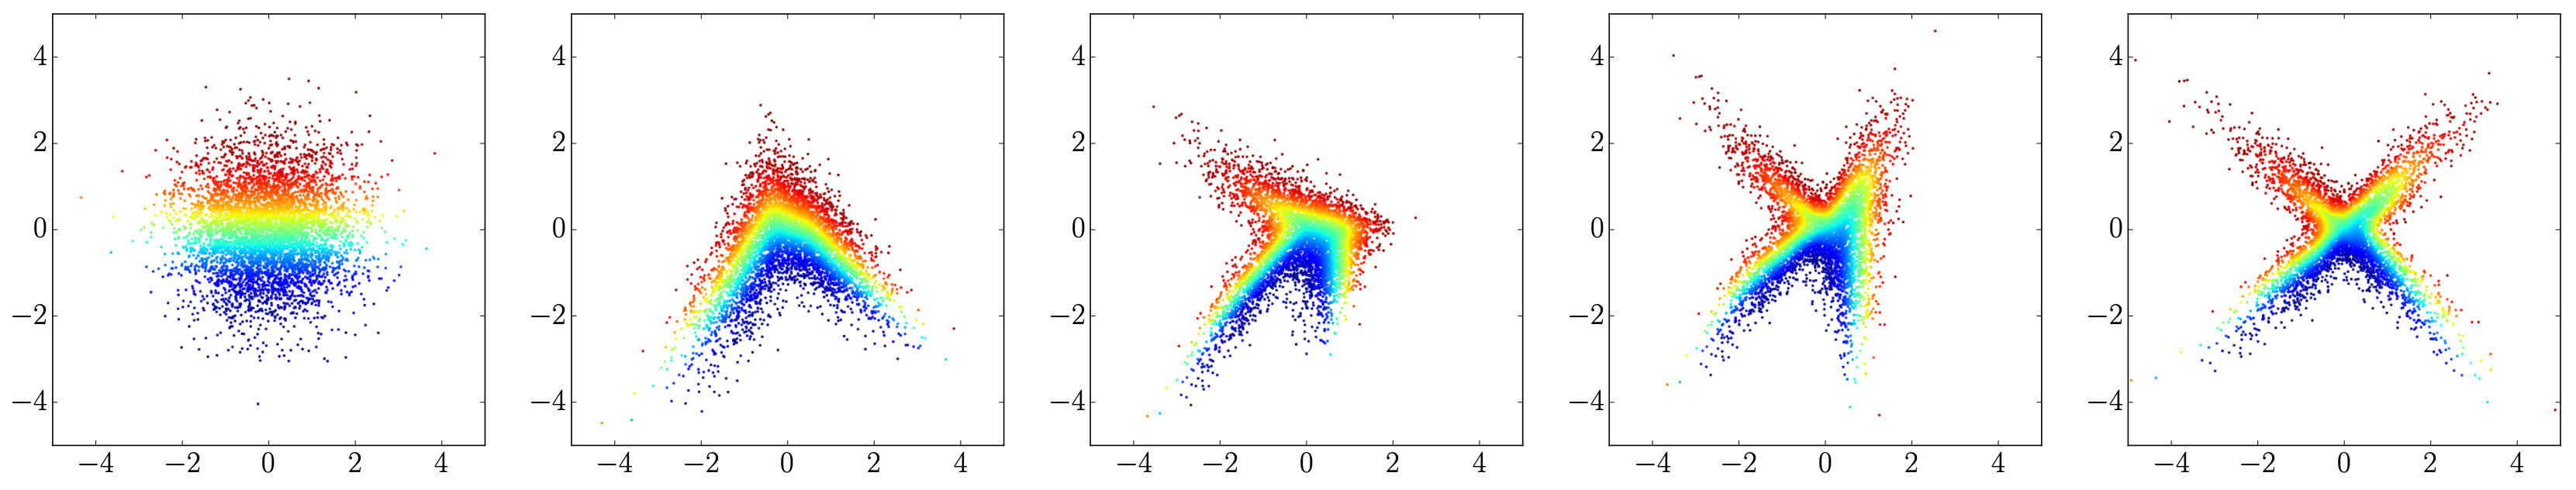
\includegraphics[width=\linewidth]{figs/flow_4_steps_example.png}
	\end{figure}
	\end{block}
	\vspace{-0.3cm}
	\begin{block}{Flow likelihood}
		\vspace{-0.3cm}
		\[
		\log p(\bx|\btheta) = \log p(f(\bx, \btheta)) + \log \left|\det \left( \frac{\partial f(\bx, \btheta)}{\partial \bx} \right) \right|
		\]
		\vspace{-0.3cm}
	\end{block}
	What is the complexity of the determinant computation?
	\begin{block}{What we want}
		\begin{itemize}
			\item Efficient computation of Jacobian $\frac{\partial f(\bx, \btheta)}{\partial \bx}$;
			\item Efficient sampling from the base distribution $p(\bz)$;
			\item Efficient inversion of $f(\bx, \btheta)$.
		\end{itemize}
		
	\end{block}
		\myfootnotewithlink{https://arxiv.org/abs/1912.02762}{Papamakarios G. et al. Normalizing flows for probabilistic modeling and inference, 2019} 
\end{frame}
%=======
\begin{frame}{Summary}
	\begin{itemize}
	\item Standart VAE has several limitations that we will address later in the course.
	\vfill
	\item Mean-field approximation is a general form of approximate variational inference.
	\vfill
	\item The EM-algorithm and VAE model can be presented as a special case of the mean-field approximation.
	\vfill
	\item Forward KL minimization is equivalent to MLE. Reverse KL is used in variational inference.
	\vfill
	\item Flow models transform a simple base distribution to a complex one via a sequence of invertible transformations.
	\vfill
	\item Flow models have a tractable likelihood that is given by the change of variable theorem.
	\end{itemize}
\end{frame}
\end{document} 